% fig_87L_fsm.tex — 87L three-mode FSM + scenario result matrix
% Compile: pdflatex fig_87L_fsm
\documentclass[tikz,border=4pt]{standalone}
\usepackage{tikz}
\usetikzlibrary{automata,positioning,arrows.meta,shapes.geometric,fit,backgrounds}

\begin{document}
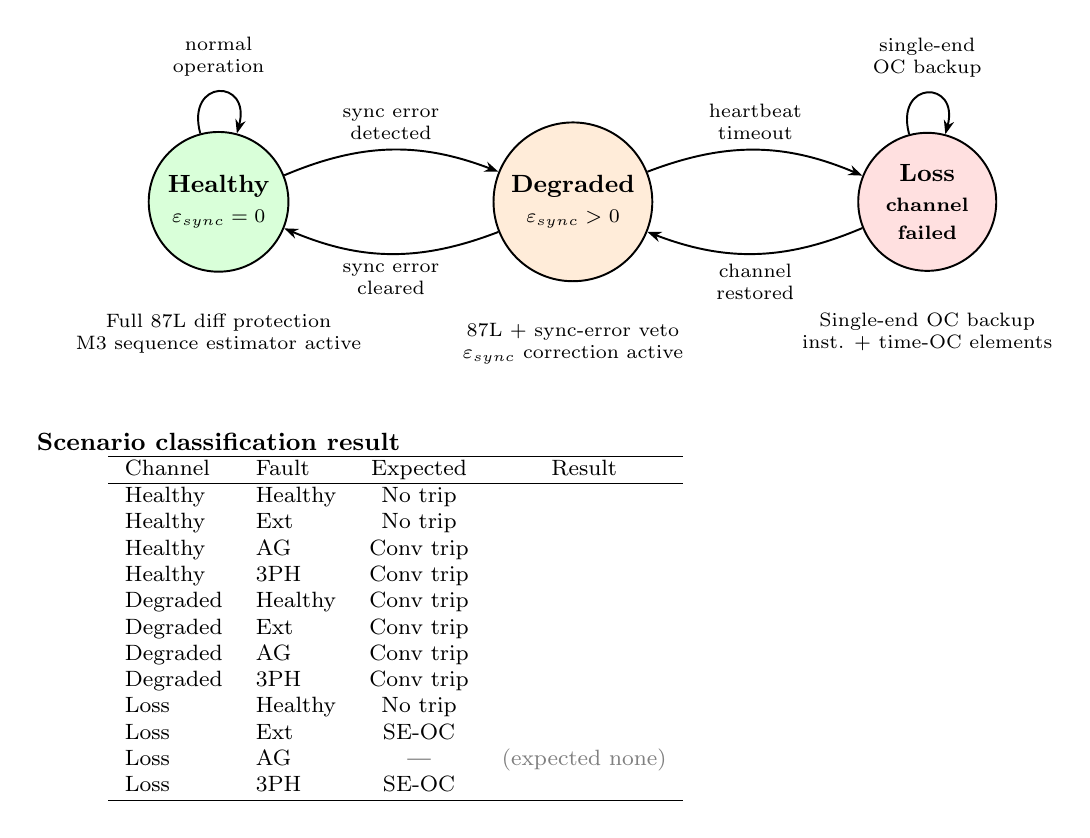
\begin{tikzpicture}[
  font=\small,
  state/.style={draw,circle,minimum size=1.6cm,align=center,
                line width=0.7pt,font=\small\bfseries},
  healthy/.style={state,fill=green!15},
  degraded/.style={state,fill=orange!15},
  loss/.style={state,fill=red!12},
  arr/.style={-{Stealth[length=5pt]},line width=0.7pt},
  translabel/.style={font=\scriptsize,align=center},
]

% ---- States -----------------------------------------------------------------
\node[healthy]  (H) at (0,0)    {Healthy\\\scriptsize$\varepsilon_{sync}=0$};
\node[degraded] (D) at (4.5,0)  {Degraded\\\scriptsize$\varepsilon_{sync}>0$};
\node[loss]     (L) at (9.0,0)  {Loss\\\scriptsize channel\\[-1pt]\scriptsize failed};

% ---- Transitions ------------------------------------------------------------
\draw[arr,bend left=22] (H) to
  node[above,translabel]{sync error\\detected} (D);
\draw[arr,bend left=22] (D) to
  node[below,translabel]{sync error\\cleared} (H);
\draw[arr,bend left=22] (D) to
  node[above,translabel]{heartbeat\\timeout} (L);
\draw[arr,bend left=22] (L) to
  node[below,translabel]{channel\\restored} (D);
\draw[arr,loop above,looseness=4] (H) to
  node[translabel,above=2pt]{normal\\operation} (H);
\draw[arr,loop above,looseness=4] (L) to
  node[translabel,above=2pt]{single-end\\OC backup} (L);

% ---- Protection action labels -----------------------------------------------
\node[font=\scriptsize,below=0.4cm of H,align=center]
  {Full 87L diff protection\\M3 sequence estimator active};
\node[font=\scriptsize,below=0.4cm of D,align=center]
  {87L + sync-error veto\\$\varepsilon_{sync}$ correction active};
\node[font=\scriptsize,below=0.4cm of L,align=center]
  {Single-end OC backup\\inst. + time-OC elements};

% ---- Result matrix ----------------------------------------------------------
\node[font=\small\bfseries, below=1.8cm of D, xshift=-4.5cm] (mtitle)
  {Scenario classification result};

% Table node (manual)
\node[below=2.2cm of H, xshift=2.25cm, anchor=north] (tbl) {
\footnotesize
\begin{tabular}{llcc}
\hline
Channel & Fault & Expected & Result \\
\hline
Healthy & Healthy  & No trip  & \textcolor{green!50!black}{\checkmark} \\
Healthy & Ext      & No trip  & \textcolor{green!50!black}{\checkmark} \\
Healthy & AG       & Conv trip & \textcolor{green!50!black}{\checkmark} \\
Healthy & 3PH      & Conv trip & \textcolor{green!50!black}{\checkmark} \\
Degraded & Healthy & Conv trip & \textcolor{green!50!black}{\checkmark} \\
Degraded & Ext     & Conv trip & \textcolor{green!50!black}{\checkmark} \\
Degraded & AG      & Conv trip & \textcolor{green!50!black}{\checkmark} \\
Degraded & 3PH     & Conv trip & \textcolor{green!50!black}{\checkmark} \\
Loss     & Healthy & No trip  & \textcolor{green!50!black}{\checkmark} \\
Loss     & Ext     & SE-OC    & \textcolor{green!50!black}{\checkmark} \\
Loss     & AG      & ---      & \textcolor{gray}{(expected none)} \\
Loss     & 3PH     & SE-OC    & \textcolor{green!50!black}{\checkmark} \\
\hline
\end{tabular}};

\end{tikzpicture}
\end{document}
